\documentclass{article}
\usepackage[T1]{fontenc}
\usepackage{lmodern}
\usepackage{graphicx}
\usepackage{amsmath,amssymb}
\usepackage[a4paper,margin=2cm]{geometry}
\usepackage[absolute,overlay]{textpos}
\setlength{\TPHorizModule}{1mm}
\setlength{\TPVertModule}{1mm}
\usepackage[indonesian]{babel}
\usepackage{hyperref}
\setlength{\emergencystretch}{2em}
% unit: Halaman 3

\begin{document}

% === Halaman 3 (llm) ===

\vspace{112.86mm}

\begin{itemize}
    \item Algoritma ini didasarkan pada persoalan \textit{Knapsack Problem}:
\end{itemize}

\vspace{20mm}

Diberikan bobot \textit{knapsack} adalah $M$. Diketahui $n$ buah objek yang masing-masing bobotnya adalah $w_1, w_2, ..., w_n$. Tentukan nilai $b_i$ sedemikian sehingga

\[ M = b_1w_1 + b_2w_2 + ... + b_nw_n \eqno(1) \]

yang dalam hal ini, $b_i$ bernilai 0 atau 1. Jika $b_i = 1$, berarti objek $i$ dimasukkan ke dalam \textit{knapsack}, sebaliknya jika $b_i = 0$, objek $i$ tidak dimasukkan.

% deskripsi: Ilustrasi Knapsack Problem yang menunjukkan tas ransel dengan kapasitas 15 kg dan beberapa objek kotak dengan label harga ($) dan berat (kg) yang berbeda-beda.
% bbox normalisasi: [0.7400, 0.0200, 0.9800, 0.4000]
\begin{textblock*}{50.40mm}(155.40mm,5.94mm)
\noindent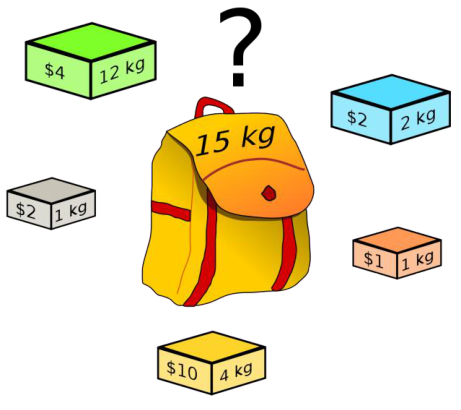
\includegraphics[width=50.40mm,height=112.86mm]{../../images/llm/page_003_img_01.png}%
\end{textblock*}

\end{document}
